\documentclass[a4paper, 12pt, oneside]{book}

\pagestyle{myheadings}

\usepackage[T1]{fontenc}
\usepackage{ae}
\usepackage[utf8]{inputenc}
\usepackage[brazilian]{babel}
\usepackage{graphicx}
\usepackage{hyperref}
\usepackage{physics}
\usepackage[export]{adjustbox}
\usepackage{float}

\linespread{1.5} 
\setlength{\hoffset}{-1in}
\setlength{\oddsidemargin}{3.0cm} 
\setlength{\textwidth}{160mm} 
\setlength{\parindent}{1.25cm} 
\setlength{\voffset}{-1in}
\addtolength{\voffset}{2.0cm}
\setlength{\topmargin}{0.0cm}
\setlength{\headheight}{5mm}
\setlength{\headsep}{5mm}
\setlength{\textheight}{247mm} 

%%%%%% COMPLETAR DADOS AQUI %%%%%%%%%%%
\def\titulo{Simulando Algoritmos Quânticos em um
Computador Clássico}
\def\tituloEN{Simulating Quantum Algorithms in a clássical
Computer}
\def\nome{Igor Valente Blackman}
\def\ano{2017}

\begin{document}

%%%%%%%%%%%%%%%%%%%%%%%%%%%%%%%%%%%%%%%%%%%%%%%
%     CAPA

\begin{titlepage}
 \noindent 
 \rule{\textwidth}{1ex} \\ [1ex]
 \begin{center}
  \begin{minipage}{0.15\textwidth}
   
\includegraphics[width=1\textwidth]{./logoUFF.png} 
  \end{minipage}
  \begin{minipage}{0.65\textwidth}
   \centering
   {\large \textsc{Universidade Federal Fluminense} } \\ [1.5ex]
   {\large \textsc{Instituto de Computação} } 
  \end{minipage}
  \begin{minipage}{0.15\textwidth}
   
\includegraphics[width=1\textwidth]{./logoIC.png}
  \end{minipage}
    
  \vfill
  {\Huge \textbf{\titulo}} \vfill
  {\huge \nome} \\ [25ex]
  {\large NITERÓI - RJ} \\ [1.5ex]
  {\large \ano}
 \end{center}\vspace{1ex}
 \rule{\textwidth}{1ex}
\end{titlepage}

%%%%%%%%%%%%%%%%%%%%%%%%%%%%%%%%%%%%%%%%%%%%%%%
%    CONTRA - CAPA

\begin{titlepage}
  \begin{center}
    \Large{\textsc{Universidade Federal Fluminense} \\
           \textsc{Instituto de Computação} \\ 
           \textsc{Departamento de Ciência da Computação} 
          }
    \par\vfill
    \LARGE{\nome}
    \par\vfill
    \LARGE{\titulo}
    \par\vfill
    \Large{NITERÓI - RJ \\
    \ano}
  \end{center}
\end{titlepage}

\pagenumbering{roman}
\setcounter{page}{2}

%%%%%%%%%%%%%%%%%%%%%%%%%%%%%%%%%%%%%%%%%%%%%%%
%    FOLHA DE ROSTO

\begin{center}

\MakeUppercase{\nome}

\vfill

\MakeUppercase{\titulo}

\vspace{3.0cm}

\begin{flushright}
\begin{minipage}{0.50\textwidth}

Trabalho submetido ao Curso de Bacharelado em Ciência da Computação da Universidade Federal Fluminense como requisito parcial para a obtenção do título de Bacharel em Ciência da Computação.

\end{minipage}
\end{flushright}

\vspace{3.0cm}

Orientadora: Profa. Dra. Karina Mochetti de Magalhães

\vfill

Niterói - RJ \\
\ano

\end{center}

\newpage

%%%%%%%%%%%%%%%%%%%%%%%%%%%%%%%%%%%%%%%%%%%%%%%%%%%%%    FICHA CATALOGRÁFICA

\newpage

%%%%%%%%%%%%%%%%%%%%%%%%%%%%%%%%%%%%%%%%%%%%%%%%%%%%%    FOLHA DE APROVAÇÃO

\newpage

%%%%%%%%%%%%%%%%%%%%%%%%%%%%%%%%%%%%%%%%%%%%%%%%%%%%%    DEDicatória

\begin{flushright}
\begin{minipage}{0.5\textwidth}

\vspace{15.0cm}

\emph{
Dedicatória
}

\end{minipage}
\end{flushright}

%%%%%%%%%%%%%%%%%%%%%%%%%%%%%%%%%%%%%%%%%%%%%%%%%%%%%    AGRADECIMENTOS

\chapter*{Agradecimentos}
\addcontentsline{toc}{chapter}{Agradecimentos}

\thispagestyle{myheadings}

\noindent

Agradecimento 1.

\ \\ 

Agradecimento 2.

\ \\ 

...

\ \\ 

Agradecimento N.

%%%%%%%%%%%%%%%%%%%%%%%%%%%%%%%%%%%%%%%%%%%%%%%%%%%%%    RESUMO

\chapter*{Resumo}
\addcontentsline{toc}{chapter}{Resumo}

\thispagestyle{myheadings}

A construção de um computador quântico terá impactos profundos em várias áreas, tais como Física, Matémática e, especialmente, a Ciência da Computação. As dificuldades práticas para se construir um computador quântico são muitas, logo não é possível prever quando ou mesmo se um computador quântico será construído. Apesar disso, a teoria na área da computação quântica vem evoluindo fortemente e para auxiliar na análise desses algoritmos pode ser essencial a criação de um simulador quântico de fácil acesso. Esse simulador utilizaria um computador clássico para realizar os trabalhos de um computador quântico, simulando o entrelaçamento e a sobreposição em bits clássicos e realizando uma estimativa de tempo gasto num computador quântico. O objetivo desse trabalho é realizar a implementação de um simulador para algoritmos quânticos.

\ \\

Palavras-chave: PALAVRA1, PALAVRA2, PALAVRA3. 

%%%%%%%%%%%%%%%%%%%%%%%%%%%%%%%%%%%%%%%%%%%%%%%%%%%%%    ABSTRACT

\chapter*{Abstract}
\addcontentsline{toc}{chapter}{Abstract}

\thispagestyle{myheadings}

The construction of a quantum computer will have deep impacts in several áreas, such as Physics, Mathematics, and especially Computer Science. There are several practical difficulties in building a quantum computer, so it is not possible to predict when or even if a quantum computer will be built. Nevertheless, the theory in the Quantum Computing field is evolving strongly and to assist in the analysis of these algorithms can be essential to creaté a quantum simulator. This simulator would be implemented in a classic computer, performing the work of a quantum computer, simulating the superposition and entanglement in clássical bits with an estimaté of efficiency. Therefore, the aim of this work is implement a simulator for quantum algorithms.

\ \\

Keywords: WORD1, WORD2, WORD3.

%%%%%%%%%%%%%%%%%%%%%%%%%%%%%%%%%%%%%%%%%%%%%%%%%%%%%    SUMן�½RIO

\tableofcontents

\thispagestyle{myheadings}

%%%%%%%%%%%%%%%%%%%%%%%%%%%%%%%%%%%%%%%%%%%%%%%%%%%%%    LISTA DE FIGURAS

\listoffigures
\addcontentsline{toc}{chapter}{Lista de Figuras}

\thispagestyle{myheadings}

%%%%%%%%%%%%%%%%%%%%%%%%%%%%%%%%%%%%%%%%%%%%%%%%%%%%%    LISTA DE TABELAS

\listoftables
\addcontentsline{toc}{chapter}{Lista de Tabelas}

\thispagestyle{myheadings}

%%%%%%%%%%%%%%%%%%%%%%%%%%%%%%%%%%%%%%%%%%%%%%%%%%%%%    TEXTO

\pagebreak
\pagenumbering{arabic}

\chapter{Introdução}
\thispagestyle{empty}

A computação quântica aproveita a possibilidade de que as particulas subatômicas podem ter mais de um estado a qualquer momento~\cite{wiredQC}. Em um computador normal, que chamaremos de clássico, um bit é um simples pedaço de informação que possui apenas dois estados, 0 ou 1. Para representar tal informação um computador deve conter algum tipo de sistema físico com dois estados distintos para associar aos valores como, por exemplo um switch que pode estar fechado (1) ou aberto (0)~\cite{mermin}.

Computadores quânticos utilizam bits quânticos ou "qubits", sistemas quânticos que também possuem dois estados, entretanto, diferente do bit clássico qubits podem armazenar muito mais informação já que eles podem existir em qualquer sobreposição desses valores, 0 ou 1, ou ambos ao mesmo tempo~\cite{wiredQC}. 

No mundo da mecânica quântica os eventos são governados por probabilidades. Um átomo radioativo, por exemplo, pode enfraquecer emitindo um eletron, ou não. É possível preparar um experimento de tal forma que exista uma chance exata de 50\% de que um dos átomos de um pedaço de matérial radioativo caia em um determinado tempo~\cite{gribbin}.

Pode-se tomar como exemplo o experimento teórico do "Gato de Schrödinger". São colocados um gato, um frasco de veneno e uma fonte de radiação em uma caixa selada. Se um monitor interno (ex. Contador Geiger) detecta radiação, o frasco é quebrado soltando o veneno, matando o gato. No mundo clássico existe uma chance de 50\% de o gato estar morto, e sem olhar dentro da caixa podemos dizer que o gato está vivo ou morto. Segundo a teoria, nenhuma das duas possibilidades tem qualquer realidade a menos que seja observada~\cite{gribbin}. Isso se equivale para o qubit, ele pode ser 0 ou 1 ao mesmo tempo mas quando ele é observado ele deixa de ser um bit quântico e passa a ser um bit clássico, ou seja, só pode ser 0 ou 1.

Outra visão quanto a um qubit pode-se pensar em uma esfera imaginaria onde um bit clássico pode estar apenas em um dos polos da esfera e o qubit, bit quântico, pode estar em qualquer ponto da esfera. Assim qubits podem armazenar uma quantidade muito maior de informação que um bit clássico.

\section{Motivação e Objetivo}

A computação quântica é uma área de pesquisa muito relevante, pois utiliza elementos de três áreas importantes: como a Física, Matémática e Engenharia. Apesar de ainda não ser possível prever quando ou mesmo se um computador quântico será construído, caso isto ocorra serão gerados grandes impactos em todas essas áreas. Em um computador quântico, os sistemas não devem ter interações físicas que não sejam sob o controle total e completo do programa. Diferente de como ocorre em um computador comum, ou os chamados computadores clássicos, interações físicas não controladas introduziriam interrupções potencialmente catastróficas na operação de um computador quântico, o que resulta numa dificuldade na construção do mesmo. 

Entretanto, os benefícios que podem ser gerados com a construção de um computador quântico vão muito além do que os pesquisadores podem imaginar. Para os cientistas da computação, o mais impressionante na computação quântica e a eficiência alcançada por seus algoritmos, algo não possível na teoria clássica da complexidade computacional. O tempo de execução de algumas tarefas em um computador quântico cresce de forma muito mais lenta com o tamanho da entrada do que em um computador clássico. 

Neste trabalho apresentamos a implementação de um simulador de circuitos quânticos que utiliza um computador clássico para executar os algoritmos em um computador quântico. Assim, características quânticas como o entrelaçamento e a sobreposição serão realizadas em bits clássicos o que resultará num gasto de tempo maior. Por isso, o simulador também gera uma estimativa de tempo gasto a partir das portas quânticas, emulando o que seria obtido por um computador quântico caso ele seja construído. As portas e o tempo gasto em cada uma e dado pelo usuário. O simulador é uma ferramenta online e dispõe de arraste das portas quânticas para formação dos circuitos com o intuito de facilitar a interação com o usuário.

\section{Revisão Bibliográfica}

\subsection{Quantum - Davy Wybiral}

Existe um simulador online desenvolvido por Davy Wybiral de Austin Texas, Quantum ou como está no projeto dele do Git Quantum Circuit Simulator~\cite{davyw}. O projeto foi disponibilizado no Git em Janeiro de 2017~\cite{gitdavyw}. Davy Wybiral utiliza o Canvas para gerar toda a parte gráfica dos circuitos e menus, e javascript para toda a parte de cálculo. O simulador não possui nenhum tipo de documentação e tem uma interface bem simples com um menu superior onde existem algumas opções e uma área com as portas quânticas que podem ser adicionadas nos circuitos e ter a quantidade dos mesmos alterada.

\begin{figure}[hbtp]
\centering
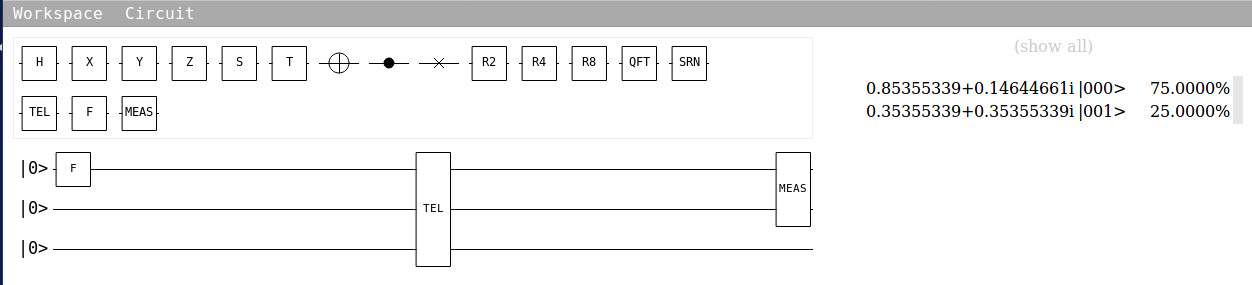
\includegraphics[scale=0.36]{davyw.jpg}
\caption{Simulador quântico de Davy Wybiral}
\end{figure}

A montagem do circuito funciona com a seleção de uma das portas e após isso basta clicar nos circuitos para adicionar a porta selecionada. Pode-se deletar uma porta clicando com o botão direito. Nos casos de portas de 2-bits é necessário que haja uma ação de clique e arraste onde o clique seleciona a posição do bit de controle e ao largar fica a porta. Existe também a possibilidade de arrastar com uma porta de 1-bit selecionada o que adiciona a mesma em diversos circuitos.

Para efetuar o cálculo do circuito basta pressionar a tecla Enter ou selecionar no menu a opção Evaluaté. O resultado é mostrado ao lado direito com todas as possibilidades possíveis e suas respectivas probabilidades.

\subsection{Quirk - Craig Gidney}

O projeto teve seu início em Março de 2014 mas não teve commits após o mes de criação. Em Novembro do mesmo ano, 2014, voltou a ter commits e entre Março de 2016 e Novembro de 2016 foi quando se teve a maior concentração de commits, 647 dos 1006 totais. O projeto ainda vem sendo atualizado sendo o commit mais recente do dia 29 de Abril de 2017~\cite{gitquirk}. Craig Gidney, desenvolvedor do Quirk, explica que decidiu criar o simulador porque ficou interessado em computação quântica e pelo fato de ter lido "Media for Thinking the Unthinkable" de Bret Victor onde ele menciona benefícios do feedback imediato em relação ao entendimento e produtividade. Craig diz não ter achado nenhum simulador de circuitos quânticos que passasse essa experiência de "manipulação direta"~\cite{quirk}. Foi desenvolvido utilizando Webgl.

\begin{figure}[hbtp]
\centering
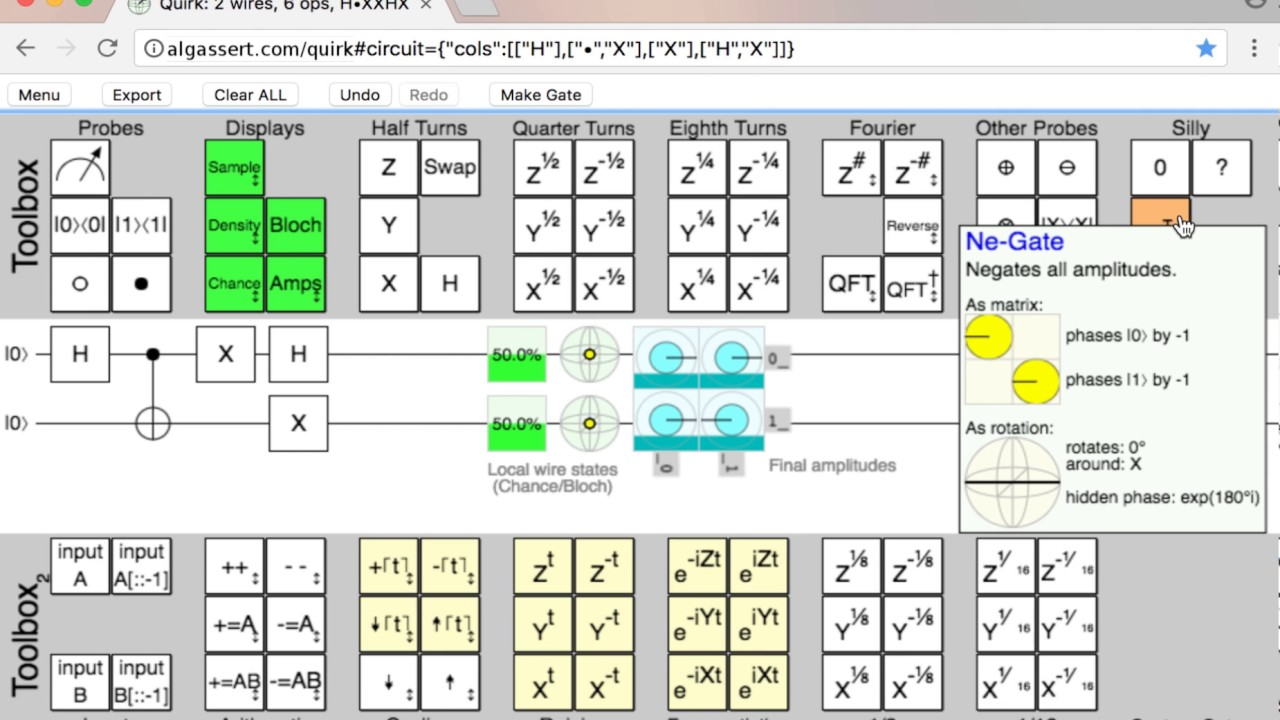
\includegraphics[scale=0.36]{quirk.jpg}
\caption{Simulador quântico Quirk de Craig Gidney}
\end{figure}

Craig faz comparações com alguns simuladores como por exemplo o já mencionado de Davy Wybiral e o IBM Quantum Experience. Ele também menciona alguns outros como Quantum Computing Playground e Microsoft's LIQ Ui|>.

O simulador Quirk é composto por um menu que possui opções de carregar alguns exemplos de circuitos já prontos, exportar o circuito montado, desfazer ou refazer alguma alteração e inclusive criar porta. Ele possui uma área com as opções de portas a serem utilizadas no circuito, formas de mostrar o resultado e mais diversas opções. Algumas vantagens desse simulador são: as portas são colocadas da forma "arrastar e soltar", o resultado é mostrado a todo momento não havendo a necessidade de se apertar um botão para isso, e é possível adicionar mais bits ao circuito dinâmicamente com o arrastar de uma das portas para além da linha do último bit.

\section{Organização do Texto}

Este trabalho está divido da seguinte forma: a Seção 2 é apresentada a motivação; na Seção 3 é realizada uma revisão bibliográfica, expondo a teoria e os frameworks existentes atualmente; a Seção 4 apresenta a solução implementada; a Seção 5 traz os resultados obtidos com o trabalho; e por final na Seção 6 são apresentadas as conclusões e trabalhos futuros.


%%%%%%%%% Circuitos Quanticos
\chapter{Circuito Quântico}

Primeiramento vamos relembrar um pouco de circuitos lógicos. Os circuitos são formados por portas como AND, OR e NOT que recebem uma sequência de valores binários 0 e 1. Ao passar pelas portas é gerada uma saída que é a entrada transformada pelo circuito.

\section{Qubit}
Já um bit quântico, ou seja um qubit, é um vetor de dois números complexos que chamaremos de a e b.
\begin{equation} \label{eq1} 
\ket{\Psi} = \mqty(a\\b).
\end{equation}

Ao ser medido os elementos $\abs{a}^2$ e $\abs{b}^2$ são, respectivamente, a probabilidade de que o qubit seja $\ket{0}$ e $\ket{1}$. 
\begin{equation} \label{eq2}
  \ket{0} = \mqty(1\\0) ,\hspace{2cm} 
  \ket{1} = \mqty(0\\1).
\end{equation}
Sendo assim os valores a e b devem seguir a regra de normalização
\begin{equation}\label{eq3}
\abs{a}^2 + \abs{b}^2 = 1,
\end{equation}
\begin{equation}\label{eq4}
\ket{\Psi} = a\ket{0} + b\ket{1} = \mqty(a\\b).
\end{equation}
O estado $\ket{\Psi}$ é dito de estar em superposição dos estados $\ket{0}$ e $\ket{1}$ com amplitudes \textit{a} e \textit{b}. Se a ou b for 0 e o outro for 1, por exemplo, é o caso especial onde o estado do qubit é igual a um dos estados classicos $\ket{0}$ ou $\ket{1}$. (pagina 17)

\section{Entrelaçamento}
Assim como o estado geral de um único qubit é qualquer superposição normalizada \eqref{eq4} dos dois possíveis estados clássicos, o estado geral de $\ket{\Psi}$ nos possibilita associar com dois qubits em qualquer superposição dos quatro estados clássicos,
\begin{equation}\label{eq5}
  \ket{00} = \mqty(1\\0\\0\\0) \hspace{1cm} 
  \ket{01} = \mqty(0\\1\\0\\0) \hspace{1cm} 
  \ket{10} = \mqty(0\\0\\1\\0) \hspace{1cm} 
  \ket{11} = \mqty(0\\0\\0\\1)
\end{equation}
\begin{equation}\label{eq6}
\ket{\Psi}_2 = a\ket{00} + b\ket{01} + c\ket{10} + d\ket{11} = \mqty(a\\b\\c\\d)
\end{equation}
Se tivermos dois qubits $\ket{\Psi} = a\ket{0} + b\ket{1}$ e $\ket{\Phi} = c\ket{0} + d\ket{1}$, então o estado $\ket{\Psi}_2$ do par é o produto tensor deles,
\begin{equation}\label{eq7}
\ket{\Psi}_2 = \ket{\Psi}\otimes\ket{\Phi} = \mqty(a \vdot c\\a \vdot d\\b \vdot c\\b \vdot d)
\end{equation}\
Assim os valores das quatro amplitudes devem seguir a regra de normalização, onde
\begin{equation}
\abs{a}^2 + \abs{b}^2 + \abs{c}^2 + \abs{d}^2 = 1
\end{equation}
Com \eqref{eq7} temos
\begin{align}
\abs{a \vdot c}^2 + \abs{a \vdot d}^2 + \abs{b \vdot c}^2 + \abs{b \vdot d}^2 \\
\abs{a}^2 \vdot \abs{c}^2 + \abs{a}^2 \vdot \abs{d}^2 + \abs{b}^2 \vdot \abs{c}^2 + \abs{b}^2 \vdot \abs{d}^2 \\
\abs{a}^2 \vdot (\abs{c}^2 + {d}^2) + \abs{b}^2 \vdot (\abs{c}^2 + \abs{d}^2) \\
\abs{a}^2 \vdot 1 + \abs{b}^2 \vdot 1 \\
\abs{a}^2 + \abs{b}^2 = 1
\end{align}
Essa relação não se mantém, e o estado geral de 2-qubit é diferente do estado geral de 2 bits clássicos, ele não é um produto \ref{eq7} de dois estados de 1-qubit. Esse estado de dois ou mais qubits é chamado de entrelaçamento.

\section{Portas quânticas}
Portas quânticas são operações básicas que podemos realizar em qubits. Essas portas podem ser representadas graficamente através de circuitos ou matemáticamente por matrizes.
\begin{equation}
\ket{\Psi'} =  U\ket{\Psi}
\qquad 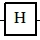
\includegraphics[width=0.07\linewidth, valign=c]{h.jpg}
\end{equation}
Uma porta quântica deve sempre ser representada por uma matriz unitária porque ao multiplicar o vetor pela matriz a norma do vetor é mantida.
\subsection{NOT} 
A operação NOT quântica faz com que as amplitudes do qubits se invertam.
\begin{equation}
X =  \mqty(0&1\\1&0)
\qquad 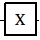
\includegraphics[width=0.07\linewidth, valign=c]{x.jpg}
\end{equation}
\begin{equation}
X\ket{\Psi} = \mqty(0&1\\1&0)\mqty(a\\b) = \mqty(0 \vdot a+1 \vdot b \\1 \vdot a+0 \vdot b) = \mqty(b\\a) = \ket{\Psi'}
\end{equation}

\subsection{Y e Z} 
Análogas a operação NOT temos as operações Y e Z.
\begin{equation}
Y =  \mqty(0&-i\\i&0)
\qquad 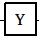
\includegraphics[width=0.07\linewidth, valign=c]{y.jpg}
\end{equation}
\begin{equation}
Z =  \mqty(1&0\\0&-1)
\qquad 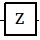
\includegraphics[width=0.07\linewidth, valign=c]{z.jpg}
\end{equation}

\subsection{Identidade} 
A operação Identidade quântica mantém os valores iniciais do qubit.
\begin{equation}
I =  \mqty(1&0\\0&1)
\qquad 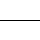
\includegraphics[width=0.07\linewidth, valign=c]{line.jpg}
\end{equation}
\begin{equation}
I\ket{\Psi} = \mqty(1&0\\0&1)\mqty(a\\b) = \mqty(1 \vdot a+0 \vdot b \\0 \vdot a+1 \vdot b) = \mqty(a\\b) = \ket{\Psi'}
\end{equation}

\subsection{Hadamard} 
A porta Hadamard é uma operação fundamental na computação quântica e não possui uma operação clássica equivalente. Ela transforma  os qubits bases $\ket{0}$ e $\ket{1}$ para um estado de sobreposição onde $\ket{0}$ e $\ket{1}$ possuem a mesma probabilidade.
\begin{equation}
H =  \frac{1}{\sqrt{2}}\mqty(1&1\\1&-1)
\qquad 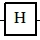
\includegraphics[width=0.07\linewidth, valign=c]{h.jpg}
\end{equation}
\begin{equation}
H\ket{\Psi} = \frac{1}{\sqrt{2}}\mqty(1&1\\1&-1)\mqty(a\\b) = \frac{1}{\sqrt{2}}\mqty(1 \vdot a+1 \vdot b \\1 \vdot a-1 \vdot b) = \mqty( \frac{a+b}{\sqrt{2}} \\ \frac{a-b}{\sqrt{2}} ) = \ket{\Psi'}
\end{equation}

\subsection{CNOT} 
A operação CNOT possui um controle. Dados dois qubits, x e y, a matriz C mantém o valor de y caso x seja igual a 0 e caso x seja igual a 1 ela inverte o valor de y.
\begin{equation}
C =  \mqty(1&0&0&0\\0&1&0&0\\0&0&1&0\\0&0&0&1)
\qquad 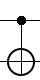
\includegraphics[width=0.07\linewidth, valign=c]{cnot.png}
\end{equation}
\begin{equation}
C\ket{\Psi} = \mqty(1&0&0&0\\0&1&0&0\\0&0&1&0\\0&0&0&1)\mqty(a\\b\\c\\d) = 
\mqty(1 \vdot a+0 \vdot b +0 \vdot c +0 \vdot d \\
	  0 \vdot a+1 \vdot b +0 \vdot c +0 \vdot d \\
	  0 \vdot a+0 \vdot b +0 \vdot c +1 \vdot d \\
	  0 \vdot a+0 \vdot b +1 \vdot c +0 \vdot d ) 
= \mqty(a\\b\\d\\c) = \ket{\Psi'}
\end{equation}

\subsection{Medição}
Quando um qubit passa pela operação de medição ele se torna um bit clássico, 0 ou 1, e por esse motivo essa operação é muito importante na computação quântica. Para fazer essa diferenciação entre qubit e bit clássico em um circuito lógico quântico, um traço representa um qubit e um traço duplo um bit clássico.
\begin{align}
\qquad 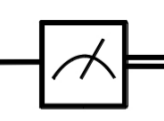
\includegraphics[width=0.1\linewidth, valign=c]{medicao.png}
\end{align}

\subsection{Código Superdenso}

Apesar que uma quantidade infinita de informações é necessária para especificar o estado $\ket{\Psi}=a\ket{0}+b\ket{1}$ de um único qubit, não existe um modo de que alguém que tenha adquirido um qubit possa descobrir qual é seu estado. Se Alice prepara um qubit no estado $\ket{\Psi}$ e envia para Bob, tudo que ele pode fazer é aplicar uma transformação unitária à sua escolha e fazer a medição do qubit, chegando ao valor 0 ou 1. O máximo que Alice pode comunicar para Bob enviando um único qubit é um único bit de informação.

E para esse problema existe o código superdenso, seu protocolo consiste de 3 usuários. Alice, que deseja enviar 2bits clássicos para Bob e Eve que fará e inicialização do sistema.

Na inicialização do sistema, Eve inicializa um qubit de tamanho dois $\ket{\Psi}=\ket{\Psi' \Psi''}$ com zero. 
\begin{equation}
\ket{\Psi} = \ket{00} = \ket{0}\otimes \ket{0} = \mqty(1\\0) \otimes \mqty(1\\0) = \mqty(1\\0\\0\\0)
\end{equation}
Após isso Eve aplica a operação Hadamard em $\ket{\Psi'}$
\begin{align}
H \otimes I = \mqty(\frac{1}{\sqrt{2}}&\frac{1}{\sqrt{2}}\\
				\frac{1}{\sqrt{2}}&-\frac{1}{\sqrt{2}} ) 
	\otimes \mqty(1&0\\0&1) 
= \mqty(\frac{1}{\sqrt{2}}\mqty(1&0\\0&1) & \frac{1}{\sqrt{2}}\mqty(1&0\\0&1) \\ 
	\frac{1}{\sqrt{2}}\mqty(1&0\\0&1) & -\frac{1}{\sqrt{2}}\mqty(1&0\\0&1))
	\\
H \otimes I = 
\mqty(\frac{1}{\sqrt{2}}&0&\frac{1}{\sqrt{2}}&0\\
	0&\frac{1}{\sqrt{2}}&0&\frac{1}{\sqrt{2}} \\
	\frac{1}{\sqrt{2}}&0&-\frac{1}{\sqrt{2}}&0 \\
	0&\frac{1}{\sqrt{2}}&0&-\frac{1}{\sqrt{2}}) \hspace{2cm} \\
(H \otimes I)\ket{\Psi} =  \mqty(\frac{1}{\sqrt{2}}&0&\frac{1}{\sqrt{2}}&0\\
	0&\frac{1}{\sqrt{2}}&0&\frac{1}{\sqrt{2}} \\
	\frac{1}{\sqrt{2}}&0&-\frac{1}{\sqrt{2}}&0 \\
	0&\frac{1}{\sqrt{2}}&0&-\frac{1}{\sqrt{2}}) 
	\mqty(1\\0\\0\\0) = \mqty(\frac{1}{\sqrt{2}}\\0\\ \frac{1}{\sqrt{2}}\\0)
\end{align}
e usa a porta CNOT em $\ket{\Psi}$.
\begin{equation}
C\ket{\Psi} = \mqty(1&0&0&0\\0&1&0&0\\0&0&0&1\\0&0&1&0) 
			\mqty(\frac{1}{\sqrt{2}}\\0\\ \frac{1}{\sqrt{2}}\\0)
		= \mqty(\frac{1}{\sqrt{2}}\\0\\ 0\\ \frac{1}{\sqrt{2}})
\end{equation}
Em seguida Eve envia $\ket{\Psi'}$ para Alice e $\ket{\Psi''}$ para Bob. 

Alice que deseja enviar dois bits clássicos $\ket{ab}$ para Bob, ao receber o qubit $\ket{\Psi'}$ de Eve aplica uma transformação U em $\ket{\Psi'}$ da seguinte forma:
\begin{itemize}
\item Se $\ket{ab}=\ket{00}$, então U = I.
\begin{align}
U = I\otimes I = \mqty(1&0\\0&1)\otimes\mqty(1&0\\0&1) = 
	\mqty(1&0&0&0\\0&1&0&0\\0&0&1&0\\0&0&0&1) \\
(I\otimes I)\ket{\Psi} = \mqty(1&0&0&0\\0&1&0&0\\0&0&1&0\\0&0&0&1)
	\mqty(\frac{1}{\sqrt{2}}\\0\\ 0\\ \frac{1}{\sqrt{2}}) 
	= \mqty(\frac{1}{\sqrt{2}}\\0\\ 0\\ \frac{1}{\sqrt{2}}) 
\end{align}
\item Se $\ket{ab}=\ket{01}$, então U = X.
\begin{align}
U = X\otimes I = \mqty(0&1\\1&0)\otimes\mqty(1&0\\0&1) = 
	\mqty(0&0&1&0\\0&0&0&1\\1&0&0&0\\0&1&0&0) \\
(X\otimes I)\ket{\Psi} =  \mqty(0&0&1&0\\0&0&0&1\\1&0&0&0\\0&1&0&0) 
	\mqty(\frac{1}{\sqrt{2}}\\0\\ 0\\ \frac{1}{\sqrt{2}}) 
	= \mqty(0\\ \frac{1}{\sqrt{2}}\\ \frac{1}{\sqrt{2}}\\ 0)\label{eq34}
\end{align}
\item Se $\ket{ab}=\ket{10}$, então U = Z.
\begin{align}
U = Z\otimes I = \mqty(1&0\\0&-1)\otimes\mqty(1&0\\0&1) = 
	\mqty(1&0&0&0\\0&1&0&0\\0&0&-1&0\\0&0&0&-1) \\
(Z\otimes I)\ket{\Psi} =  \mqty(1&0&0&0\\0&1&0&0\\0&0&-1&0\\0&0&0&-1) 
	\mqty(\frac{1}{\sqrt{2}}\\0\\ 0\\ \frac{1}{\sqrt{2}}) 
	= \mqty(\frac{1}{\sqrt{2}}\\0\\ 0\\ -\frac{1}{\sqrt{2}}) 
\end{align}
\item Se $\ket{ab}=\ket{11}$, então U = XZ.
\begin{align}
U = XZ\otimes I = \mqty(1&1\\1&-1)\otimes\mqty(1&0\\0&1) = 
	\mqty(1&0&1&0\\0&1&0&1\\1&0&-1&0\\0&1&0&-1) \\
(XZ\otimes I)\ket{\Psi} =  \mqty(1&0&1&0\\0&1&0&1\\1&0&-1&0\\0&1&0&-1)
	\mqty(\frac{1}{\sqrt{2}}\\0\\ 0\\ \frac{1}{\sqrt{2}}) 
	= \mqty(\frac{1}{\sqrt{2}}\\ \frac{1}{\sqrt{2}}\\ \frac{1}{\sqrt{2}}\\ -\frac{1}{\sqrt{2}}) 
\end{align}
\end{itemize}
Depois de aplicada a transformação, Alice envia $U\ket{\Psi'}$ para Bob. Para continuar as equações usaremos $\ket{ab}=\ket{01}$ \eqref{eq34}.

Bob aplica a porta CNOT em $\ket{\Psi}$
\begin{equation}
C\ket{\Psi} = \mqty(1&0&0&0\\0&1&0&0\\0&0&0&1\\0&0&1&0) 
			\mqty(0\\ \frac{1}{\sqrt{2}}\\ \frac{1}{\sqrt{2}}\\0)
		= \mqty(0\\ \frac{1}{\sqrt{2}}\\ 0\\ \frac{1}{\sqrt{2}}),
\end{equation}
em seguida usa a porta Hadamard em $U\ket{\Psi'}$
\begin{align}
H \otimes I = \mqty(\frac{1}{\sqrt{2}}&\frac{1}{\sqrt{2}}\\
				\frac{1}{\sqrt{2}}&-\frac{1}{\sqrt{2}} ) 
	\otimes \mqty(1&0\\0&1) 
= \mqty(\frac{1}{\sqrt{2}}&0&\frac{1}{\sqrt{2}}&0\\
	0&\frac{1}{\sqrt{2}}&0&\frac{1}{\sqrt{2}} \\
	\frac{1}{\sqrt{2}}&0&-\frac{1}{\sqrt{2}}&0 \\
	0&\frac{1}{\sqrt{2}}&0&-\frac{1}{\sqrt{2}}) \\
(H \otimes I)\ket{\Psi} =  \mqty(\frac{1}{\sqrt{2}}&0&\frac{1}{\sqrt{2}}&0\\
	0&\frac{1}{\sqrt{2}}&0&\frac{1}{\sqrt{2}} \\
	\frac{1}{\sqrt{2}}&0&-\frac{1}{\sqrt{2}}&0 \\
	0&\frac{1}{\sqrt{2}}&0&-\frac{1}{\sqrt{2}}) 
	\mqty(0\\ \frac{1}{\sqrt{2}}\\ 0\\ \frac{1}{\sqrt{2}}) = \mqty(0\\1\\0\\0)
\end{align}
que recebeu de Alice. Após tudo isso Bob faz a medição dos dois qubits, passando eles para bits clássicos $\ket{ab}$
\begin{align}
\ket{\Psi} = \mqty(0\\1\\0\\0) \hspace{2.5cm} \\
\ket{\Psi} = 0\vdot\ket{00} + 1\vdot\ket{01} + 0\vdot\ket{10} + 0\vdot\ket{11} \\
\ket{ab} = \ket{01}. \hspace{2.5cm}
\end{align}
(pagina 149)
\begin{figure}[H]
\centering
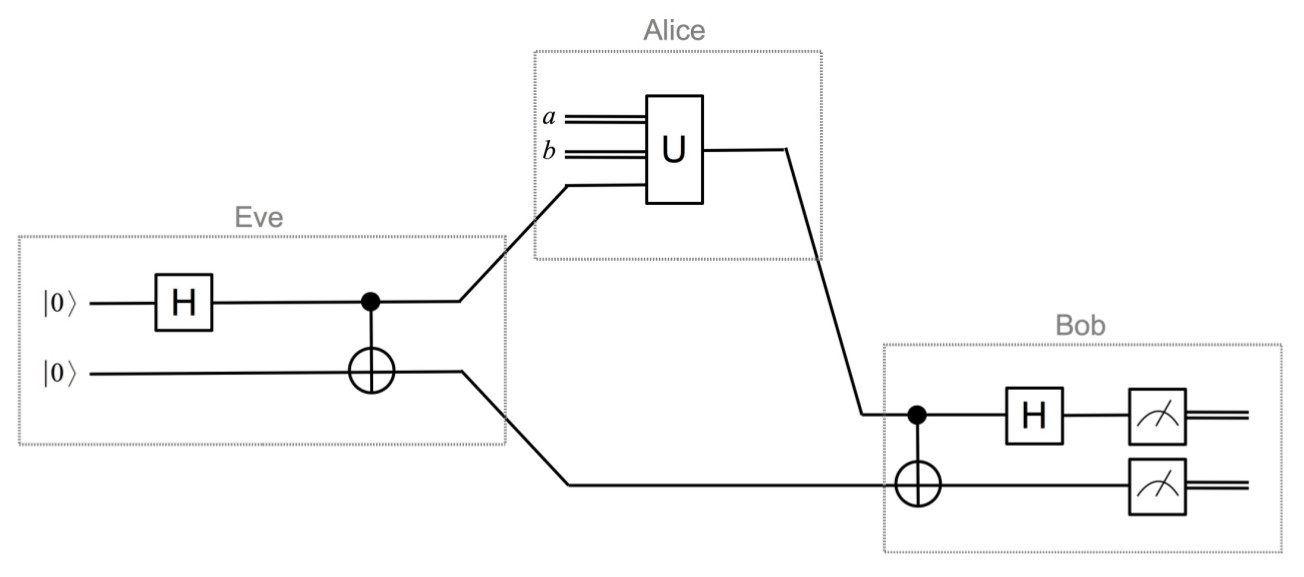
\includegraphics[scale=0.38]{superdenso.jpg}
\caption{Código Superdenso}
\end{figure}


%%%%%%%%%%%%% Escolha das ferramentas
\chapter{Escolha das ferramentas}
\thispagestyle{empty} 


Neste capítulo iremos falar sobre as opções e escolhas de linguagem, biblioteca e frameworks para desenvolvimento do proejto. 

\section{Linguagem}

Python foi a escolha por possuir todos os requisitos necessários para o desenvolvimento do projeto, frameworks de desenvolvimento web e bibliotecas de circuitos quânticos. Além disso, ela é vastamente utilizada em diversas aplicações e empresas como YouTube, Google, Industrial Light e Magic~\cite{pythonquotes} o que adiciona mais valor ao seu aprendizdo.

\section{Biblioteca}

Tendo em vista que escolhemos python como linguagem agora é a vez de escolhermos alguma biblioteca para nos ajudar com os cálculos de cicuito quântico. A seguir falamos sobre algumas opções encontradas e qual foi a escolhida.
\subsection{PyQu}
PyQu é um módulo de extensão para Python 3 com o objetivo principal de providenciar um completo conjunto de tipos de dados e funções para simular computação quântica com uma sintaxe pura. Entretanto o último commit feito foi há 7 anos o que nos fez entender que o projeto foi descontinuado, fazendo com que discartassemos essa opção~\cite{pyqu}.

\subsection{Qitensor}
Qitensor outro módulo que essencialmente é um pacote para Numpy~\cite{numpy}, utiliza semânticas mais úteis para mecânica quântica de dimensões finitas de muitas partículas. Infelizmente essa biblioteca também não recebia atualizações há mais de ano~\cite{qitensor}.
\subsection{Qubiter}
Qubiter tem como intuíto ajudar no designer e simulação de circuitos quânticos em computadores clássicos. É um projeto gêmeo do Quantum Fog e eles esperam que um dia o Quantum Fog chame o Qubiter para realizar algumas tarefas, como compilação e simulação quântica~\cite{qubiter}.	

\subsection{QuTiP}
QuTiP teve sua primeira versão em Julho de 2011~\cite{qutipchangelog}. É um software open-source para simular as dinâmicas de um sistema quântico aberto que utiliza os pacotes numéricos Numpy, Scipy e Cython. Teve sua primeira versão em Julho de 2011. Possui também um output gráfico provido pela Matplotlib. QuTiP tem como objetivo providenciar simulações numéricas eficientes e amigáveis para o usuário de um variado numero de Hamiltonianas comumente achadas em uma vasta quantidade de aplicações físicas. Está disponível sem custos para Linux, Mac OSX e Windows, sendo esta última com algumas restrições~\cite{qutip.org}. \cite{teste}

\subsection{Escolhida}
QuTip foi a escolhida por possuir pacotes numéricos e também output gráfico, mesmo este último não tendo sido utilizado no projeto mas com ele existe a possibilidade de utilização em trabalhos futuros. Além de possuir a melhor documentação dentre as bibliotecas pesquisadas, com exemplos e tutoriais.

\section{Framework Web}
Frameworks web são projetados para dar suporte no desenvolvimento de sites dinâmicos, aplicações web e web services, auxiliando no trabalho de tarefas comuns como, controle de sessão, validação de dados, acesso ao banco de dados, templates, tratamento de requisições e respostas HTTP, etc. Dentre os frameworks web existentes para python avaliamos neste trabalho Flask, Pyramid e Django.
\subsection{Flask}
Flask é o framework mais recente encontrado, foi criado em meados de 2010. Evoluiu muito a partir da análise de framworks anteriores e tem se destacado em pequenos projetos. A sua comunidade é pequena se comparada a do Django mas é ativa em listas de email e no IRC~\cite{ryanbrown}. 

\subsection{Pyramid}
O Pyramid foi criado a partir do projeto Pylons~\cite{pylonsproject} e recebeu o nome de Pyramid somente no ano de 2010, mesmo tendo sua primeira realease em 2005. É um framework tão maduro quanto o Django e disponibiliza mais flexibilidade para desenvolvedores que possuem projetos onde o caso de uso não se encaixe muito bem nos padrões do mapeamento objeto-relacional, que nada mais é do que a representação das tabelas do banco de dados através de classes onde cada resgistro é representado como uma instancia da classe~\cite{pyramid}. Pode-se dizer que Pyramid é o framework mais flexível dentre os estudados. Apesar disso, pareceu muito mais complexo do que noso projeto necessitava. Além disso ele possui a comunidade mais inativa dentre os frameworks pesquisados.

\subsection{Django}
Django foi lançado em 2005. É um framework com foco em grandes aplicações que inclui dezenas de extras para lidar com as tarefas comuns do desenvolvimento web, como por exemplo autenticação e administração de conteúdo, além de auxiliar também com questões de segurança como SQL injection com seus querysets, evitar ataques Cross Site Scripting e fornecer proteção a Clickjacking~\cite{django}. Sem dúvida o Django é o framework mais popular e a lista de sites que o utilizam é impressionante, tendo mais de 5000 páginas~\cite{listadjangosites}. Para sites que possuem requisitos comuns, Django segue padrões bem sensatos tornando-o uma escolha bem popular entre aplicações web de porte médio ou grande.

\subsection{Comunidade}
Django possui uma quantidade enorme de perguntas no StackOverflow se comparado com os outros dois Frameworks, Django 144.000, Flask 16.600, Pyramid 1.900 (Maio 2017)~\cite{stackoverflowtags}. Já no Github Flask e Django têm números semelhantes e Pyramid 10 vezes menos, Flask possui um pouco mais de 27.200 estrelas, Django pouco mais de 25.900 e Pyramid 2.300~\cite{github}. Esses números evidenciam a populariedade e o suporte oferecido por cada framework.

\subsection{Escolhido}
O Flask seria uma boa opção entretanto escolhemos o Django por:
\begin{itemize}
\item possuir uma grande comunidade ativa;
\item diversas ferramentas já inclusas, evitando o tempo de reprogramação de funções comuns;
\item ser facilmente escalável, pensando em uma futura continuação deste Proejto Final
\item ser uma ferramenta muito utilizada no mercado, trazendo mais benefícios com o aprendizado.
\end{itemize}


%%%%%%%%%%%%%%% Desenvolvimento
\chapter{Desenvolvimento}
\thispagestyle{empty} 

\section{Construção da Pagina}
A ideia inicial do simulador era de termos uma área com os inputs de tempo, as portas e o circuito. No início do desenvolvimento já fomos definindo um pouco melhor onde deveríamos ter o que. Como um dos objetivos do projeto é de simular o tempo que um computador quântico levaria para executar o circuito decidimos por colocar os inputs em primeiro lugar, ficando assim a esquerda e em cima. 

Já pensando sobre a área para montar o ciruito resolvemos que as portas ficariam em cima pois ao carregar a página o circuito estaria vazio e para que ao mesmo tempo essa parte se diferenciasse dos inputs resolvemos colocá-la a direita.

Por final precisamos de uma área para mostrar o resultado o que fez total sentido em deixá-la depois de tudo pois ela seria dependente das anteriores, sendo assim ficou na parte de baixo de tudo.

\begin{figure}[H]
\centering
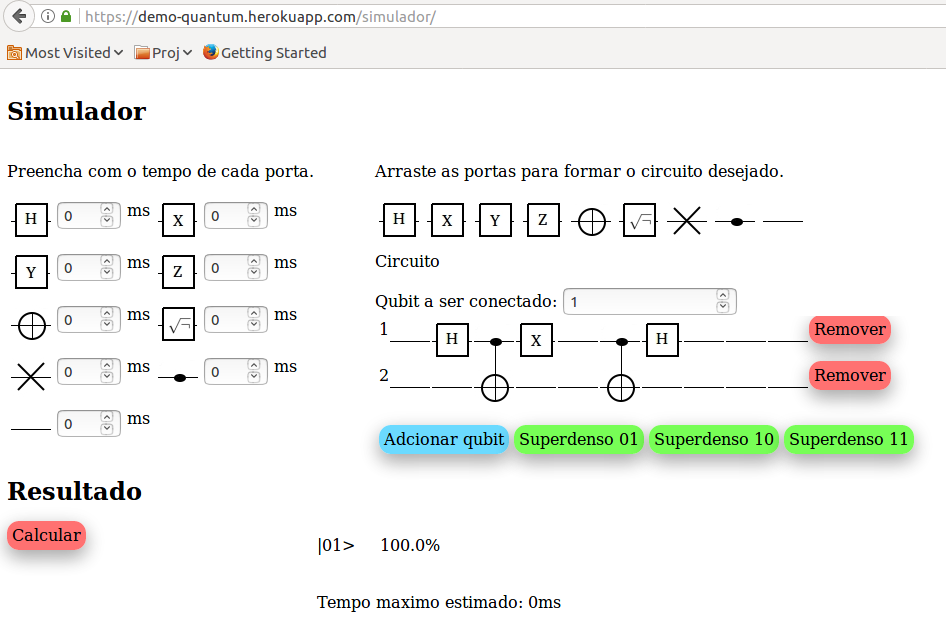
\includegraphics[scale=0.4]{simulador-pagina.png}
\caption{Nosso simulador circuito quântico online}
\end{figure}

\section{Arquiterura}

Escolhemos o padrão Model-View-Controller (MVC) para o projeto até porque o Django já segue esse padrão e que faz muito sentido para o desenvolvimento de aplicações online.

Esse estilo arquitetural é composto de três elementos: modelo, visão e controle. O modelo é composto dos elementos que representam os principais conceitos do domínio, se pensarmos na orientação a objetos, o modelo seria as classes do sistema e que normalmente são persistidas em bancos de dados. Mas não possuem nenhum acesso de fora do sistema. Já a visão é composta por elementos de interface com o usuário, podendo ser uma interface gráfica, linha de comando ou uma API que manipulam elementos do modelo. E por últimos mas não menos importante o controle que são elementos responsáveis pela orquestração, que manipulam uma visão e executam os casos de uso.

No MVC uma visão conhece seu modelo mas o modelo não conhece sua visão, os controles conhecem suas visões mas a visão não conhece seu controle. E as entidade do modelo não conhecem ninguém a não ser as outras entidades do modelo.

\begin{figure}[H]
\centering
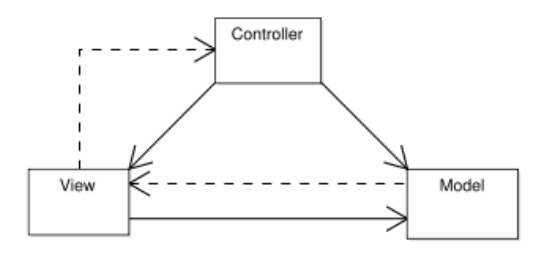
\includegraphics[scale=0.4]{mvc.png}
\caption{Diagrama MVC \cite{mvc-murta}}
\end{figure}

Vantagens do MVC:
\begin{itemize}
\item responsabilidades bem definidas por componente
\item modularização da aplicação, o que traz idependência 
\item fácil manutenabilidade
\item alta reutilização
\item possibilita desenvolvedores trabalharem simultaneamente
\end{itemize}

\section{Django e MVC}
O Django possui uma peculiaridade, ele utiliza o padrão Model View Controller (MVC) entretanto possui nomes peculiares para seus componentes. Para a parte de modelo ele chama de ``model'' e para View de ``template'' até então tudo bem, mas quando chega na parte do Controller ele chama de ``view'' o que gera confusão e reclamações de muitos. No próprio site do Django~\cite{django} existe uma pergunta sobre isso onde eles respondem que ``view'' representa os dados que são apresentados ao usuário, não necessariamente como é apresentado. Então para eles a ``view'' representa qual informação é vista e ``template'' como ela é vista~\cite{django-mvc}.

\section{Drag and Drop}

Como o simulador deveria ser amigável para o usuário decidimos utilizar Drag \& Drop (D\&{D}) para a criação/edição do circuito. Resolvemos que o simulador deveria ter uma área com as portas quânticas disponíveis para montar o circuito quântico e a partir dessa área o usuário poderia arrastar as portas para formar o circuito. Entretanto os D\&{D} convencionais apenas possibilitavam o arrastar de um elemento para um outro container, ou seja, o elemento deixava de existir no container original e era adicionado no final. O que queriamos era que o elemento inicial continuasse existindo onde estava e que uma cópia do mesmo fosse criada e adicionada ao container alvo, ou final, por isso decidimos criar um.

Sendo assim utilizamos Javascript e JQuery~\cite{jquery}, uma biblioteca de JS, para criar uma cópia do elemento que sofreu o evento de Drag e movemos a cópia até o destino do Drop. E ao realizar o Drop existe uma checagem para excluir o elemento existente e adicionar a cópia. Nos materias encontrados sobre D\&{D} o elemento utilizado pelo Javascript para capturar o elemento do drop era o ev.target o que gera alguns problemas pois esse target não traz especificamente o elemento com o evento de drop atrelado, podendo trazer uma das divs que o encapsulam ou algum outro elemento mais interno fazendo com que não houvesse uma consistencia do retorno. Para resolver esse problema decidimos utilizar currentTarget ao invés do target.

Quando pensamos nas portas de 2 qubits nos deparamos com outro problema. Como iríamos fazer a seleção do qubit de controle? A escolha foi ter um input que serviria de alvo do segundo qubit e a partir disso bastou fazer o tratamento para quando o alvo era igual ao bit do Drop ou caso o alvo fosse maior que o número de bits. No primeiro caso é solto um alerta com a mensagem de que não se pode arrastar a parta para o mesmo bit alvo da conexão, e no segundo caso o alvo se torna o último qubit do circuito ou o primeiro caso o valor seja negativo.

\section{Cálculo via Ajax}

Ajax, ou JavaScript e XML assíncronos, não é uma lingaguem e sim uma combinação de técnicas que utilizam ferramentas já embutidas do browser para realizar requisições ao servidor e receber respostas do mesmo de forma assíncrona, sem a necessidade de recarregar a página inteira, apenas parte da mesma.

A escolha do Ajax para realização do cálculo se deve ao simples fato de que o simulador tem o intuito de ser amigável ao usuário e dessa forma utilizando Ajax não existe a necessidade de recarregar a pagina ou ser direcionado para uma outra.

Primeiramente existe o tratamento do circuito para um objeto de fácil acesso à aplicação onde decidimos por utilizar JSON (JavaScript Object Notation - Notação de Objetos JavaScript) que é uma formatação de dados fácil de ler e escrever para pessoas, e fácil de interpretar e gerar para computadores. JSON é composto por duas estruturas:
\begin{itemize}
\item Uma coleção de pares nome/valor;
\item Uma lista ordenada de valores.
\end{itemize}
Por serem estruturas de dados comuns a todas as linguagens é uma ótima opção de formato para troca de dados~\cite{json}.

Após isso colocamos os elementos, as portas, pertencentes ao circuito em um array de arrays, a quantidade de qubits que o circuito possui, as conexões entre as portas e enviamos tudo para o servidor.

Agora pela parte do servidor por estarmos utilizando o Django, ele já trata essa parte de requisição e respostas~\cite{django-req-resp}. Dentro da view, que é considerado um controle pelo Django, bastou pegar o objeto Request fazer a leitura do JSON que foi enviado pelo AJAX e trabalhar em cima dele utilizando a bibliotéca QuTip para realizar o cáculo.

A parte do cálculo do tempo por não necessitar da bibliotéca ou qualquer outra informação por parte do servidor poderia ser feita na própria pagina pelo JavaScript, pois as únicas informações necessárias eram os inputs de tempo de cada porta e que portas formavam o circuito.

Ao receber o retorno do servidor, o AJAX adiciona os resultados, tanto o do cálculo do circuito quanto o do cálculo do tempo, na área do HTML de resultados da página.

\section{Usando QuTip}

Utilizar a bibliotéca QuTip se mostrou um desafio maior do que imaginávamos. Entretanto após aprender a usá-la a mesma se torou uma excelente ferramenta. QuTip possui alguns objetos, um deles é o QubitCircuit que representa um programa/algoritmo quântico que mantém uma sequência de Gates, estes últimos são representações das portas quânticas. O QubitCircuit possui uma função add\_gate com os seguintes parâmetros:
\begin{itemize}
\item gate - Nome da porta, dentro de uma lista aceitável. RX, RY, RZ, CRX, CRY, CRZ, SQRTNOT, SNOT, PHASEGATE, CPHASE, CNOT, CSIGN, BERKELEY, SWAPalpha, SWAP, ISWAP, SQRTSWAP, SQRTISWAP, FREDKIN, TOFFOLI, GLOBALPHASE;
\item targets - Uma lista com os qubits alvos;
\item controls - Uma lista com os qubits de controle;
\item arg\_value - Parâmetro para a transformação, do tipo Float;
\item arg\_label - Label para representação da porta.
\end{itemize}
Dependendo da porta desejada para adicionar no circuito alguns dos parâmetros viram obrigatórios. Como por exemplo para adicionar a porta Hadamard basta qcircuit.add\_gate(``SNOT'', targets=[0]).

Após montarmos o objeto QubitCircuit com as portas passadas no Request. Deve-se calcular a matriz de propagação e para isso existe a função QubitCircuit.propagators() que faz esse cáculo retornando uma lista com os passos em forma de matrizes unitárias operando da esquerda para a direita. Agora com essa lista é chamada a função gate\_sequence\_product() passando a lista como parâmetro que retorna a matriz unitária final gerada a partir de uma lista de operações unitárias. 

O objeto gerado pela função gate\_sequence\_product() é então multiplicado pelo vetor coluna dos qubits passados no input que para o projeto assumimos que sempre são $\ket{0}$. Essa multiplicação gera outro vetor coluna com as probabilidades dos valores finais para o circuito e é nesse vetor que é feito uma análise para retirada legível dos resultados que são retornados para o AJAX.

\section{Hospedagem - Heroku}

Como o simulador tem o objetivo de ser online utilizamos a plataforma da nuvem Heroku para a hospedagem. O Heroku é um PaaS (Platform as a Service) que faz com que o desenvolvedor não tenha que se preocupar com infraestrutura tendo assim foco total no desenvolvimento, sem precisar gerenciar, fazer a manutenção e garantir a segurança do servidor~\cite{heroku}. Ele possui uma opção grátis que da suporte a diversas linguagem sendo uma delas python, o que fez dela uma escolha perfeita.

A configuração do projeto para rodar no Heroku não foi complicada. Bastou o projeto estar no Git, preparar um ambiente virtual com todas as dependências necessárias, gerar um arquivo texto chamado ``requirements.txt'' com essas dependência, o que pode ser feito com o comando ``pip freeze > requirements.txt'', adicionar esse arquivo ao diretório do projeto. Criar um outro arquivo ``runtime.txt'' para especificar a versão do python a ser utilizada. É necessário criar um ``Procfile'' que serve para declarar o comando que será executado para começar a aplicação, no caso do projeto coloquei ``web: gunicorn quantum-circuit-simulator.wsgi --log-file -''. 

Após essas configurações básicas é necessário criar uma conta no Heroku e instalar o Heroku CLI. Com a instalação do Heroku CLI podemos executar o comando ``heroku login'' e entrar com as credenciais de login. Após isso entrar com o comando ``heroku create nome-aplicacao'', adicionar e commitar todas as alterações feitas no projeto e fazer o deploy da aplicação no Heroku ``git push heroku master''.

Durante o deploy o Heroku:
\begin{itemize}
\item detecta a linguagem;
\item faz a instalção dos requisitos que estão no arquivo ``requirements.txt'';
\item roda o comando no Procfile.
\end{itemize}

Com o deploy da sua aplicação feito basta acessar a url da aplicação acessando sua conta do Heroku ou executando o comando ``heroku open''~\cite{heroku-python}.

\chapter{Resultados}
\thispagestyle{empty} 

Texto...

\chapter{Conclusão e Trabalhos Futuros}
\thispagestyle{empty} 

Texto...

%%%%%%%%%%%%%%%%%%%%%%%%%%%%%%%%%%%%%%%%%%%%%%%%%%%%%    REFERÊNCIAS BIBLIOGRÁFICAS
\bibliographystyle{plain}
\bibliography{monografia}



\end{document}


